\documentclass[a4paper]{article}
\usepackage[margin=1in]{geometry}
\usepackage{tikz}
\usepackage{slashbox}

\begin{document}

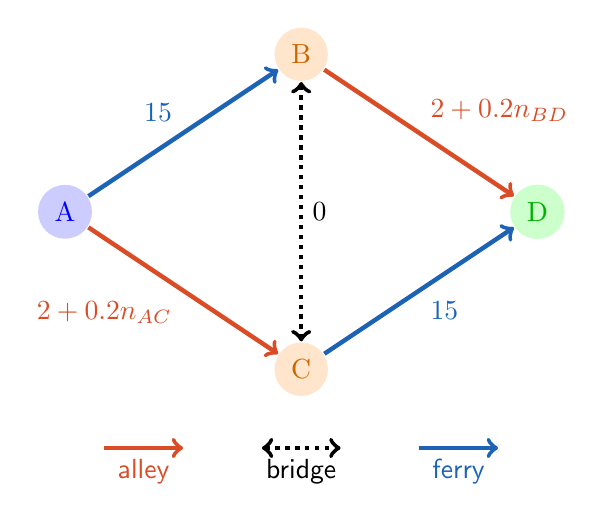
\begin{tikzpicture}
    \node (A) at (0,0) [thick, blue, circle, fill=blue!20] {A};
    \node (D) at (6,0) [thick, green!70!black, circle, fill=green!20] {D};
    \node (B) at (3,2) [thick, orange!80!black, circle, fill=orange!20] {B};
    \node (C) at (3,-2) [thick, orange!80!black, circle, fill=orange!20] {C};

    % ferry
    \draw [->, ultra thick, cyan!40!blue] (A)--(B) node[midway, anchor=south east]{15};
    \draw [->, ultra thick, cyan!40!blue] (C)--(D) node[midway, anchor=north west]{15};

    % alley
    \draw [->, ultra thick, red!40!brown] (A)--(C) node[midway, anchor=north east]{$2+0.2 n_{AC}$};
    \draw [->, ultra thick, red!40!brown] (B)--(D) node[midway, anchor=south west]{$2+0.2 n_{BD}$};

    % bridge
    \draw [<->, dotted, ultra thick] (B)--(C) node[midway,right]{0};

    \draw [->, ultra thick, red!40!brown] (0.5,-3)--(1.5,-3) node[midway, anchor = north]{\textsf{alley}};
    \draw [<->, dotted, ultra thick] (2.5,-3)--(3.5,-3) node[midway, anchor = north]{\textsf{bridge}};
    \draw [->, ultra thick, cyan!40!blue] (4.5,-3)--(5.5,-3) node[midway, anchor = north]{\textsf{ferry}};

\end{tikzpicture}

\bigskip


\newcommand{\backslashcolor}[2]{\backslashbox{\textcolor{red}{#1}}{\textcolor{blue}{#2}}}

\begin{tabular}{c|c|c|c|}
    \backslashcolor{$a_1$}{$a_2$} & Rock & Paper & Scissors \\ \hline
    Rock & \backslashcolor{0}{0} &\backslashcolor{-1}{1} & \backslashcolor{1}{-1} \\ \hline
    Paper & \backslashcolor{1}{-1} &\backslashcolor{0}{0} & \backslashcolor{-1}{1} \\ \hline
    Scissors & \backslashcolor{-1}{1} &\backslashcolor{1}{-1} & \backslashcolor{0}{0} \\ \hline
\end{tabular}






































\end{document}